\chapter{MASTER THESIS PROPOSAL}
\label{chap:proposal}

The core challenge addressed by this project is the fundamental paradox in conservation genomics: endangered species, which require the most precise genetic tools for their protection, often have the least genetic data available for analysis. Traditional approaches to geographic assignment require substantial sample sizes per population to achieve reliable results, creating a significant barrier for species like jaguars where populations are small, fragmented, and difficult to sample \cite{shafer2015genomics}.

The innovative approach proposed here leverages the power of transfer learning in machine learning to overcome this data scarcity challenge. By pre-training a foundation model on comprehensive feline genomic data and then fine-tuning it on jaguar-specific sequences, we can potentially achieve levels of precision and reliability that were previously unattainable with traditional methods. This approach represents a paradigm shift in conservation genomics, moving from methods that require large datasets to methods that can work effectively with limited data through the power of pre-trained models.

\section{OBJECTIVES}

\subsection{General Objective}

Develop and evaluate a machine learning pipeline using transfer learning and foundation models for precise geographic assignment of jaguars (\textit{Panthera onca}) from different Brazilian biomes, overcoming the limitations of limited genetic data through pre-training on comprehensive feline genomic datasets.

\subsection{Specific Objectives}

\begin{enumerate}
	\item Pre-train a DNABERT-2 foundation model on comprehensive feline genomic data from the Darwin's Ark database to learn general patterns of genomic variation across felid species;
	\item Fine-tune the pre-trained model on complete jaguar genomes from different Brazilian biomes to develop a specialized model for jaguar geographic assignment;
	\item Evaluate the performance of the transfer learning approach compared to traditional methods for geographic assignment, particularly in scenarios with limited sample sizes;
	\item Develop a computational pipeline for automated geographic assignment of jaguar samples of unknown origin, with applications in forensic analysis and conservation management;
	\item Assess the model's ability to identify subtle genetic differentiation between recently fragmented populations, particularly in the Atlantic Forest biome where sample sizes are critically small.
\end{enumerate}

\section{MATERIALS AND METHODS}

\subsection{Data Acquisition}

\subsubsection{Pre-training Dataset: Darwin's Ark Feline Genomes}

For the pre-training phase, we will utilize the comprehensive feline genomic database available through Darwin's Ark (https://darwinsark.org/). This database contains complete genome sequences from multiple felid species, providing a rich source of genomic variation across the Felidae family. The dataset includes genomes from various wild and domestic cat species, offering the foundation model exposure to diverse genomic patterns and evolutionary relationships within the felid lineage.

The Darwin's Ark database provides access to high-quality, curated genomic data that will allow the model to learn general patterns of genomic variation, sequence motifs, and evolutionary relationships that are conserved across felid species. This pre-training step is crucial for developing a robust foundation model that can later be fine-tuned for jaguar-specific applications.

\subsubsection{Fine-tuning Dataset: Jaguar Complete Genomes}

The fine-tuning dataset will consist of complete jaguar genomes available at the Laboratory of Genomic and Molecular Biology of PUCRS (LBGM-PUCRS), derived from studies related to jaguar ecology, genetics, and evolution. We will analyze at least 45 complete jaguar genomes sequenced on the Illumina HiSeq platform, with an average coverage of 46x.

These genomes were obtained from individuals sampled throughout the species' distribution in Brazil through collaboration with field researchers, including 10 individuals from the Amazon, 13 from the Atlantic Forest, 5 from the Caatinga, 12 from the Cerrado, and 5 from the Pantanal. Additional genomes may be included in the analyses as samples and/or sequences become available during the study.

\subsection{Model Architecture and Training Strategy}

\subsubsection{Foundation Model: DNABERT-2}

We will employ the DNABERT-2 architecture as our foundation model, which represents the current state-of-the-art in genomic language modeling \cite{zhou2024dnabert}.

The model incorporates several advanced architectural features designed to handle the specific complexities of genomic data. Central to its design is Attention with Linear Biases (ALiBi), a mechanism that allows the model to extrapolate to longer input sequences than those seen during training, effectively bypassing the limitations of traditional learned positional embeddings. Furthermore, the integration of Flash Attention drastically improves memory usage and computational speed during both training and inference phases. These optimizations, combined with its inherent multi-species pre-training capability, allow DNABERT-2 to learn robust, generalizable patterns across diverse genomic datasets before specific adaptation.

\subsubsection{Transfer Learning Pipeline}

To leverage the limited available jaguar data effectively, the training process will follow a rigorous two-stage transfer learning approach, moving from general feline genomic understanding to specific species-level geographic assignment.

\textbf{Stage 1: Pre-training on Feline Genomes}

The first stage involves pre-training the DNABERT-2 model on a broad dataset of feline genomes sourced from the Darwin's Ark project. This phase aims to teach the model the fundamental ``grammar'' and syntax of feline DNA. We will employ a Masked Language Modeling (MLM) objective, where 15\% of the tokens in the input sequences are randomly masked, and the model must predict the original identity of these masked tokens based on context. To ensure stable convergence and efficient learning of general features, this stage will utilize a large batch size of 4096 and a maximum sequence length of 128 base pairs.

\textbf{Stage 2: Fine-tuning on Jaguar Genomes}

The second stage focuses on fine-tuning this pre-trained model specifically for the task of geographic assignment in jaguars. In this phase, the weights learned from the broad feline dataset are adjusted using jaguar-specific genomic data. We will replace the general MLM head with a task-specific classification head designed to map genetic sequences to distinct geographic regions. To accommodate the nuances of the smaller target dataset, we will employ smaller batch sizes and reduced learning rates to prevent catastrophic forgetting of the pre-trained features. Additionally, to mitigate the risk of overfitting we will implement rigorous cross-validation strategies and apply data augmentation techniques to synthetically increase the effective size and diversity of the training set.

\subsubsection{Model Training for Geographic Assignment}

The geographic assignment task will be formulated as a regression problem, where the model predicts the latitude and longitude of origin for each jaguar genome, similar to the approach used by \textit{Locator} \cite{battey2020predicting}. This allows for finer spatial resolution than biome classification and enables targeted enforcement at critical poaching hotspots.

The training workflow begins with data preprocessing, which involves sequence quality control, normalization, and the encoding of genomic variation into model-compatible formats. Following this, we perform feature extraction using a pre-trained genomic foundation model or dimensionality reduction techniques to capture relevant genetic variation patterns. The architecture concludes with a regression head consisting of fully connected layers that output continuous latitude and longitude coordinates.

To ensure robust generalization, we apply regularization techniques such as dropout, weight decay, and early stopping to prevent overfitting. Finally, the model utilizes cross-validation with spatially aware k-fold techniques (e.g., spatial blocking) to ensure robust evaluation and avoid overestimating accuracy from geographically close samples.

\subsubsection{Performance Evaluation}

We will evaluate the model's geographic prediction performance using metrics suited for continuous spatial outputs. The primary metric is the Mean Absolute Error (MAE), which calculates the average geographic distance (in kilometers) between predicted and true coordinates. We will complement this with the Median Error Distance, a robust measure less sensitive to large outliers, and the $R^2$ Score to assess the proportion of variance in coordinates explained by the model.

Beyond scalar metrics, we will generate error distribution maps to visualize spatial bias or the clustering of errors. These evaluations will be substantiated by cross-validation scores derived from spatially aware folds. Finally, the model will be validated through a comparison with traditional methods, benchmarking against classical SNP-based assignment approaches using population clustering or frequency-based likelihood methods.

\subsection{Computational Infrastructure}

\subsubsection{Hardware Requirements}

The project will require significant computational resources for model training and evaluation. The hardware setup is centered on GPUs, specifically requiring 2 high-performance units (e.g., NVIDIA RTX 4090 or equivalent). To handle large genomic datasets, the system requires a minimum of 64GB memory (RAM) and high-speed SSD storage for efficient data access. Additionally, a multi-core CPU is necessary to handle data preprocessing and analysis workloads.

\subsubsection{Software Stack}

The computational pipeline will utilize a robust software stack anchored by Python as the primary programming language for model development. The deep learning components will be implemented using the PyTorch framework, utilizing the Transformers library specifically for DNABERT-2 model implementation. These core components will be supported by specialized bioinformatics tools for genomic data processing and various statistical packages for population genetic analyses and evaluation.

\subsection{Validation and Testing}

\subsubsection{Cross-validation Strategy}

Given the limited sample sizes, we will implement a comprehensive cross-validation strategy. We will primarily employ stratified k-fold cross-validation to ensure the representation of all biomes in each fold. In scenarios with very small sample sizes, we will utilize leave-one-out cross-validation. Furthermore, we will apply bootstrap resampling to estimate confidence intervals for model performance, providing a measure of statistical uncertainty.

\subsubsection{Independent Test Set}

We will reserve a portion of the jaguar genomes as an independent test set. This data will be excluded from training to evaluate final model performance and prevent overfitting to the training data.

\subsubsection{Comparison with Traditional Methods}

To validate our approach, we will compare the performance of our transfer learning model with traditional SNP-based geographic assignment methods, population genetic clustering approaches such as STRUCTURE \cite{pritchard2000inference} and ADMIXTURE, and distance-based assignment methods. This comparison will help quantify the advantages of the transfer learning approach, particularly in scenarios with limited data.

\section{SCHEDULE}

The project will be conducted over 12 months, with the following schedule:

\textbf{Months 1-2: Literature Review and Data Preparation}

\begin{itemize}
	\item Comprehensive review of transfer learning applications in genomics
	\item Data collection and preprocessing from Darwin's Ark database
	\item Initial setup of computational infrastructure
\end{itemize}

\textbf{Months 3-5: Pre-training Phase}

\begin{itemize}
	\item Implementation of DNABERT-2 architecture
	\item Pre-training on feline genomic data from Darwin's Ark
	\item Model validation and optimization
\end{itemize}

\textbf{Months 6-8: Fine-tuning and Model Development}

\begin{itemize}
	\item Fine-tuning on jaguar genomic data
	\item Development of geographic assignment pipeline
	\item Initial performance evaluation
\end{itemize}

\textbf{Months 9-10: Validation and Testing}

\begin{itemize}
	\item Cross-validation studies
	\item Comparison with traditional methods
	\item Performance optimization
\end{itemize}

\textbf{Months 11-12: Analysis and Documentation}

\begin{itemize}
	\item Final model evaluation
	\item Results analysis and interpretation
	\item Thesis writing and documentation
\end{itemize}

\begin{figure}[H]
\raggedright
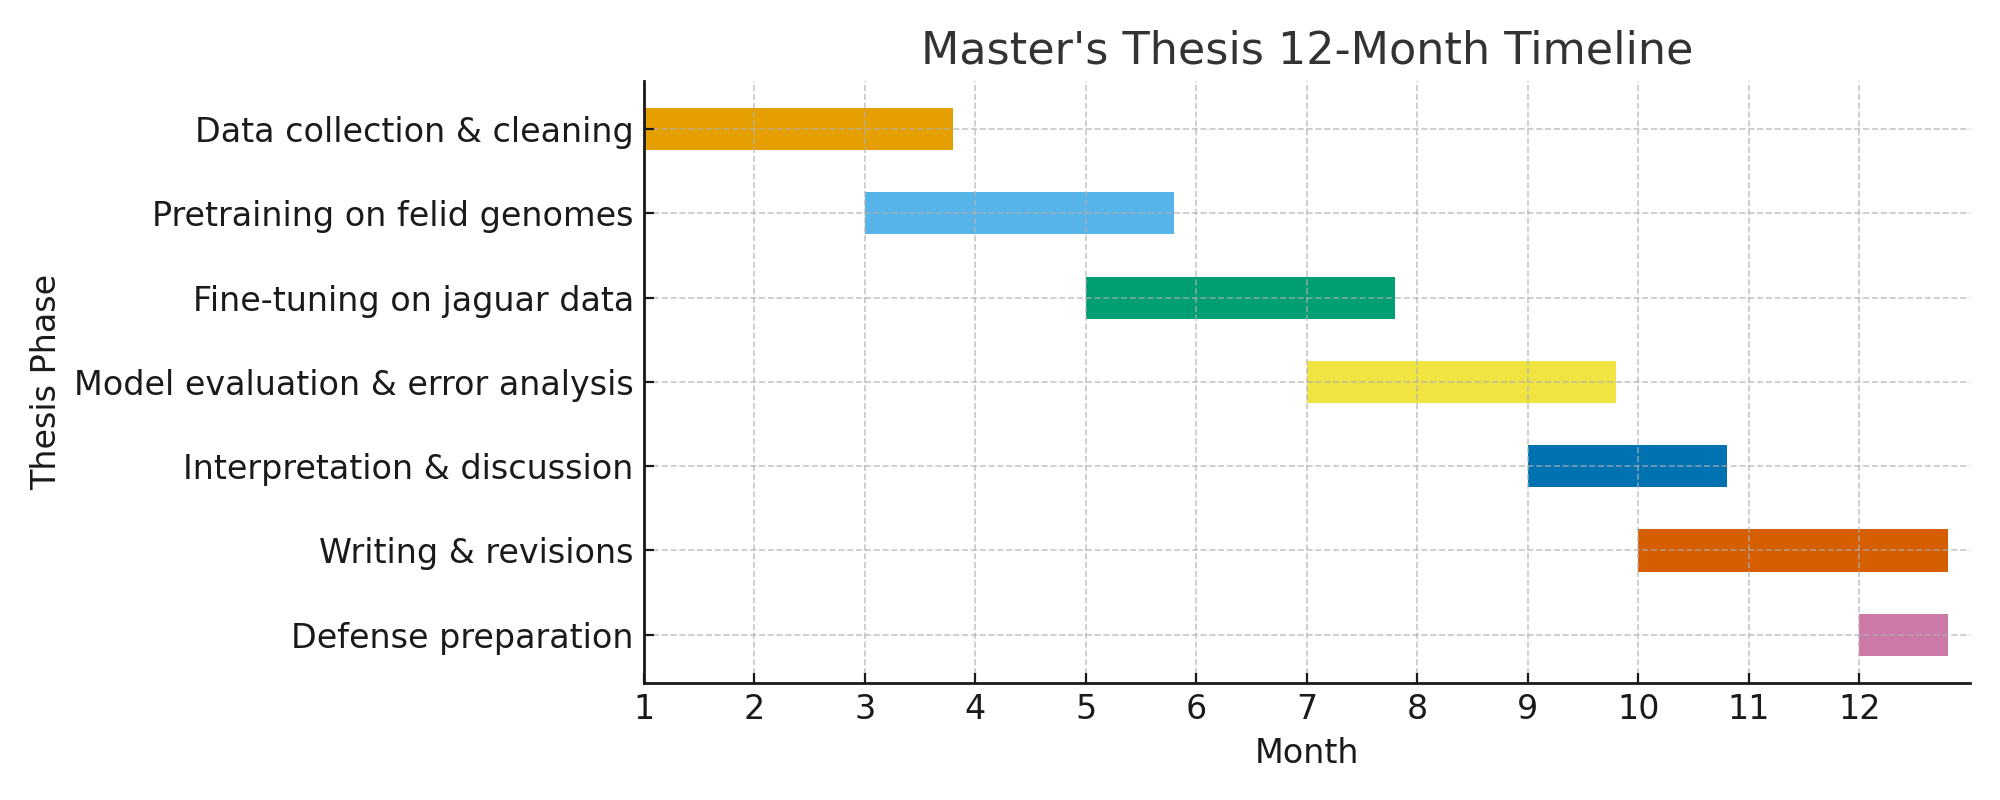
\includegraphics[width=0.9\textwidth]{images/image7.png}
\caption{Project timeline and schedule}
\label{fig:project_timeline}
\end{figure}

\section{BUDGET}

The project budget is primarily allocated to the computational resources required for model development and training. The core infrastructure necessitates two NVIDIA RTX 4090 GPUs, each equipped with 24 GB of VRAM, which are sufficient for both DNABERT-2 pretraining and jaguar fine-tuning; this component is estimated at \$2,400. To support large-scale experiments and potential tokenizer training, we have allocated \$1,200 for access to a high-performance computing cluster. Additionally, \$600 is designated for cloud computing services to ensure robust backups, validation runs, and external reproducibility.

Beyond the primary processing units, the host system requires specific specifications to maintain efficient data pipelines. We recommend at least 128 GB of host RAM; while training a BPE tokenizer from scratch typically requires over 1 TB of RAM, we mitigate this requirement by reusing the released DNABERT-2 tokenizer. Regarding local storage, a 200 GB SSD is necessary to accommodate approximately 30 GB of raw genomic corpora, up to 120 GB of tokenized datasets, rolling checkpoints, and system logs.

The total estimated budget for these resources is \$4,200. It is important to note that this figure estimates the opportunity cost of computational resources (PUCRs) rather than solely direct expenses. The proposed infrastructure aligns with the requirements reported for the 117M parameter DNABERT-2 model \cite{zhou2024dnabert}, which was originally trained on eight 2080 Ti GPUs over approximately 14 days. Our setup using two 4090 GPUs offers significantly more VRAM per card (24 GB compared to 11 GB), allowing for larger per-GPU batches or gradient accumulation to match the required throughput.

\section{EXPECTED OUTCOMES}

This project is expected to deliver:

\begin{enumerate}
	\item A novel transfer learning approach for geographic assignment in endangered species
	\item A pre-trained foundation model for felid genomics
	\item A specialized model for jaguar geographic assignment
	\item A computational pipeline for automated geographic assignment
	\item Validation of transfer learning approaches in conservation genomics
	\item Comparison framework for traditional vs. machine learning methods
\end{enumerate}

The results will contribute to both the scientific understanding of transfer learning in genomics and the practical conservation of jaguars through improved forensic and management tools.
